
\section{Introdução}

Neste trabalho será implementado um classificador logístico para classificar uma base de dados binária. Com recurso a este classificador logistico pretende-se verificar a separabilidade linear do dataset. Adicionalmente também se pretende avaliar a eficácia da técnica de pooling no reconhecimento de imagens. O pooling será analisado segundo duas vertentes, sendo a primeira a redução dimensional das imagens do dataset e a segunda a escolha de um filtro bem parametrizado que permita separar o ruido da informação útil presente na imagem. 
Em seguida explicar-se-á em que consiste a base de dados referida, o que é um classificador logístico, em que consiste o pooling e as metodologias utilizadas no mesmo.


\subsection{Base de dados}

Uma base de dados é uma sequência de eventos ($e$), a sua expressão genérica é a seguinte:
\hfill\newline
\hfill\newline
$D = (e^n)^N_{n=1}$, em que N é o número total de eventos em consideração.
\hfill\newline
\hfill\newline
Um evento ($e$) é composto por duas categorias, a primeira categoria refere-se aos dados de input ou seja aos atributos denominados $X$ e a segunda catagoria, denominada $y$, trata-se da label dado que corresponde ao output. A expressão genérica de um evento é a seguinte:
\hfill\newline
\hfill\newline
$e = (X,y)$
\hfill\newline
\hfill\newline
Tratando-se um evento de um par (imagem, label) o número total de atributos da imagem de um evento corresponde ao produto do número de linhas pelo número de colunas da mesma. Note-se ainda que como $X$ representa uma imagem cada um dos seus constituintes é um valor inteiro entre 0 e 255 que representa o nível de cinzento de um pixel.



\subsection{Classificador logístico}


A regressão logistica é um método de classificação simples e poderoso que pode ser utilizado na separação de dados binários. Um classificador logístico trata-se portanto de uma \textit{"machine learning"} cuja arquitetura permite receber na entrada um vetor $X^m$, de tamanho $I$ e devolve um valor $\hat{y}$ no domínio [0,1] representando a probabilidade dessa imagem pertencer á classe $y$, $y \in \{0,1\}$\cite{ref2,ref5}. Os seguintes passos mostram a construção da formula que corresponde a esta operação:\newline
\hfill\newline
O primeiro passo passa por definir o vetor $X^m$ como o vetor que possui os I pixeis da imagem m do dataset.\newline
\hfill\newline
$X^m=X_i^m, i=1,...,I$
\hfill\newline
\hfill\newline
O segundo passo passa por definir $\theta$ (vetor de pesos) como:\hfill\newline
\hfill\newline
$\theta = (\theta_i),i=0,...,I$
\hfill\newline
\hfill\newline
Assim, o produto de $\theta$ por $X$ pode ser definido como\cite{ref2,ref3}:\hfill\newline
\hfill\newline
 $\theta^T X = \sum_{i=1}^{I} (\theta_i X_i)$.
\hfill\newline
\hfill\newline
Desta forma a formula correspondente a esta operação fica totalmente definida como\cite{ref2}:

\hfill\newline
$\hat{y} = f(X) = \sigma(\theta_0 + \theta^T X)$, em que $\theta$ representa o vetor de pesos e $\sigma$ repesenta a função sigmoid.
\hfill\newline

Como a regressão logística prevê valores entre 0 e 1 é necessária uma função que mapeie o nosso dominio de input $\mathbb{R}$ para o dominio de output [0,1]. Esta operação é realizada recorrendo á função sigmoid que converte os valores recebidos para o dominio pretendido\cite{ref2}:
\hfill\newline
\hfill\newline
$\sigma(z) = \frac{1}{1+e^{-z}}$
\hfill\newline
\hfill\newline
As probabilidades das duas classes são portanto modeladas como \newline

$Pr\{y = 1|z\} = \frac{1}{1+e^{-z}}$\newline

e \newline

$Pr\{y = 0|z\} = 1 - \sigma(z) = \frac{e^{-z}}{1+e^{-z}}$\newline


A representação gráfica desta função pode ser vista como:

\begin{figure}[H]

  \centering
  \captionsetup{justification=centering}

  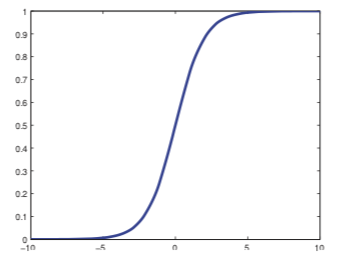
\includegraphics[width = 0.5\textwidth]{sigmoid.png}
  
  \caption {Gráfico da função sigmoid}

\end{figure}



\subsubsection{Função Custo}\hfill\newline
\hfill\newline

A função custo tem como objetivo quantificar a diferença entre o valor real e a predição. Esta função utiliza um vetor de pesos $\theta$, um vetor representativo da imagem $X$ e o valor da label associada a essa imagem $y$. Esta função começa por invocar um classificador logistico para obter uma predição $\hat{y}$. De seguida fazendo uso dos valores de $y$ e da probabilidade calculada da imagem pertencer a essa mesma classe $\hat{y}$ a diferença entre o valor real e o previsto é calculada da seguinte forma:
\hfill\newline
\hfill\newline
$E(\theta; e) = y*{\log_\epsilon (\hat{y})}+(1-y)*{\log_\epsilon (1-\hat{y})}$, em que $e$ é um evento composto por um par (X,y) respetivamente um vetor representativo de uma imagem e a label associada.

\hfill\newline
\hfill\newline
Como esta função é aplicada a toda a base de dados podemos generalizar a formula anterior para: 
\hfill\newline
\hfill\newline
$E(\theta; Base De Dados) = \frac{\sum_{n=0}^{N} y*{\log_\epsilon (\hat{y})}+(1-y)*{\log_\epsilon (1-\hat{y})}}{N}$

\hfill\newline
\hfill\newline

O vetor de pesos ($\theta$) ótimo é obtido através da minimização de uma função de custos que quantifica o erro entre a classe real e a sua predicção. O $\theta$ ideal é aquele que maximiza a probabilidade dos dados observados e denomina-se $\overline{\theta}$. \newline

\subsubsection{Atualização dos pesos}\hfill\newline
\hfill\newline

Para realizar a atualização dos pesos em classificadores logisticos é comum utilizar o método do gradiente, também chamado de método do declive que é utilizado para otimização. Para encontrar um mínimo local de uma função utiliza-se um esquema iterativo onde em cada passo se escolhe a direção negativa do gradiente a qual corresponde á direção de declive máximo. As seguintes definições explicam o processo de update dos pesos.\newline
\hfill\newline
Seja $\theta^0$ o vetor de pesos inicial e $\tau$ o learning rate usado pelo classificador logistico. Adcionalmente definimos $G$ como sendo a diferença entre o valor real $y$ e o valor da predição $\hat{y}$.\hfill\newline
\hfill\newline

$G = |y - \hat{y}|$ 
\hfill\newline
\hfill\newline

 A atualização dos pesos de $\theta^k$ para $\theta^{k+1}$ é feita então em duas etapas. A primeira atualiza a primeira componente $\theta_0$, e a segunda atualiza as restantes componentes de $\theta$\cite{ref2,ref4}.\hfill\newline
Relembrando as formulas anteriormente usadas para definir $\theta$ e o vetor de pixeis $X^m$ temos:\hfill\newline
\hfill\newline
$X^m=X_i^m, i=1,...,I$\hfill\newline
\hfill\newline
$\theta = (\theta_i),i=0,...,I$\hfill\newline
\hfill\newline
As formulas que mostram a atualização dos pesos definem-se como:\hfill\newline
\hfill\newline
$\theta_0(k+1) = \theta_0(k) + G \tau$\hfill\newline
\hfill\newline
$\theta_i(k+1) = \theta_i(k) + G \tau X_i,i=1,...,I$

\hfill\newline

Esta atualização de pesos é realizada $k$ vezes e quando $k$ tende para $\infty$, $\theta^k$ tende para $\overline{\theta}$ que corresponde ao array de pesos que minimizam o erro\cite{ref2}. Em notação simplificada:
 $k \xrightarrow{} \infty \Rightarrow \theta^k \xrightarrow{} \overline{\theta}$.\hfill\newline


%Os gráficos obtidos são do erro e função do k!! <-

\subsection{Matriz de Confusão}

A matriz de confusão é uma ferramenta muito utilizada em avaliações de modelos de previsão e é composta por quatro campos a saber\cite{ref9}:
\begin{itemize}
  \item Verdadeiro positivo (VP)\hfill\newline
  \hfill\newline
  Ocorre quando no conjunto real, a classe que pretendemos prever foi prevista corretamente.  \hfill\newline
  \item Verdadeiro negativo (VN)\hfill\newline
  \hfill\newline
  Ocorre quando no conjunto real, a classe que pretendemos prever foi prevista incorretamente.\hfill\newline
  \item Falso positivo (FP)\hfill\newline
  \hfill\newline
  Ocorre quando no conjunto real, a classe que não pretendemos prever foi prevista corretamente.\hfill\newline
  \item Falso negativo (FN)\hfill\newline
  \hfill\newline
  Ocorre quando no conjunto real, a classe que não pretendemos prever foi prevista incorretamente.\hfill\newline
\end{itemize}

A partir desta matriz podem-se calcular alguns valores importantes para avaliar a qualidade de predição do nosso modelo, esses valores são\cite{ref9}:

\begin{itemize}
  \item Accuracy\hfill\newline
  \hfill\newline
  Indica a taxa de sucesso das predições realizadas.\hfill\newline
  \hfill\newline
  $Accuracy = \frac{VP + FP}{VP+VN+FP+FN}$
  \hfill\newline
  \item Recall\hfill\newline
  \hfill\newline
  Indica a proporção de valores positivos corretamente identificados. Trata-se de uma boa métrica a aplicar em casos em que os Falsos Negativos são considerados mais prejudiciais que os Falsos Positivos.
  \hfill\newline
  \hfill\newline
  $Recall = \frac{VP}{VP+FN}$
  \hfill\newline
  \item Precisão\hfill\newline
  \hfill\newline
  Indica a percentagem de classificações positivas corretamente classificadas. Trata-se de uma boa métrica a aplicar em casos em que os Falsos Positivos são considerados mais prejudiciais do que os Falsos Negativos.
  \hfill\newline
  \hfill\newline
  $Precis\tilde{a}o = \frac{VP}{VP+FP}$
  \hfill\newpage
  \item F-score\hfill\newline
  \hfill\newline
  Esta métrica é uma média balanceada entre as métricas Recall e Precisão.
  \hfill\newline
  \hfill\newline
  $F\-score = 2*\frac{Precis\tilde{a}o * Recall}{Precis\tilde{a}o + Recall}$ 
\end{itemize}

Como exemplo de utilização desta matriz seja o array $Y$ o array de labels com os valores reais e seja $\hat{Y}$ o array de labels obtidas usando o classificador logistico, tendo ambos tamanho N. Convêm referir que caso o resultado de $\hat{y}(X^m,\theta) < 0.5$ a label $\hat{Y}_m$, correspondente á imagem $X^m$, será 0 e caso contrário será 1, uma vez que este indica a probabilidade de ser uma label e não a label em si\cite{ref2,ref3}. Assim a matriz de confusão será criada contabilizando em cada campo os valores que respeitarem as restrições apresentadas:


\begin{center}
 \resizebox{\textwidth}{!}{ %
 \begin{tabular}{||l|| c | c||} 
 \hline
 \backslashbox{Real}{Previsto} & Verdadeiro & Falso  \\ [0.5ex] 
 \hline\hline
 Verdadeiro & $Y_n == 1 \wedge \hat{Y}_n == 1, \forall n \in [0,N]$ & $Y_n == 1 \wedge \hat{Y}_n == 0, \forall n \in [0,N]$\\ 
 \hline
 Falso & $Y_n == 0 \wedge \hat{Y}_n == 1, \forall n \in [0,N]$ & $Y_n == 0 \wedge \hat{Y}_n == 0, \forall n \in [0,N]$ \\
 \hline
\end{tabular}%
  }
\end{center}




\section{Pooling}

Muitas vezes uma base de dados de imagens com imagens muito grandes (com um elevado número pixeis a serem processados) torna o processo de previsão, análise de custos e update de pesos bastante demorado\cite{ref8}.\newline
A técnica de pooling permite dividir uma imagem em várias mais pequenas através de uma janela deslizante e aplicar um filtro a cada uma de forma a remover o ruido, manter a informação útil e reduzir a dimensão da imagem a analisar\cite{ref8}.\newline
Seja $B$ uma imagem composta por pixeis a ser processada por pooling e $A$ uma janela deslizante, com dimensões inferiores a $B$, a ser usada no processo, isto é o número de pixeis da janela $A$ é inferior ao número de pixeis de $B$.\newline
O deslize da janela $A$ sobre a imagem original é determinado por um stride horizontal e um stride vertical. A cada sub-imagem obtida pela aplicação de $A$ a $B$ é posteriormente aplicado um filtro que permite obter um valor a partir dos pixeis existentes na sub-imagem, este processo denomina-se pooling. No final, juntando todos os resultados obtidos pelo filtro, obtemos uma imagem reduzida $C$ que será utilizada para realizar a classificação pretendida.\newline
Em baixo podemos visualizar, na imagem a), um exemplo da aplicação de um filtro a uma janela\cite{ref8}, já na segunda imagem apresentada é representado um exemplo da aplicação de um filtro á janela deslizante de tamanho 3x3 com um stride de 2 ao longo de uma das dimensões da imagem\cite{ref8}.

\begin{figure}[H]

  
  \captionsetup{justification=centering}
  \captionsetup{justification=centering}
  \begin{subfigure}{.5\textwidth}
  \centering
  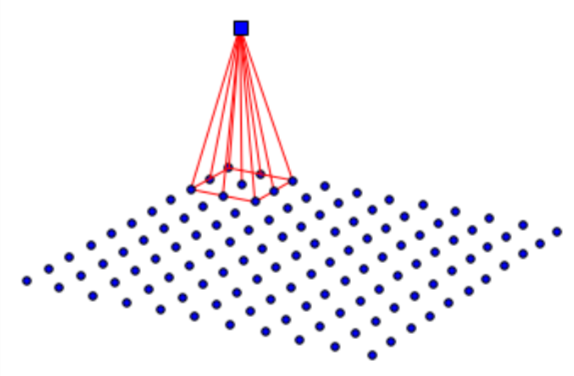
\includegraphics[width = 0.8\textwidth]{aplicacaoFiltro.png}
  \caption {Exemplo de aplicação de um filtro a uma janela sobre uma imagem representada por pixeis}
  \end{subfigure}
  \begin{subfigure}{.5\textwidth}
  \centering
   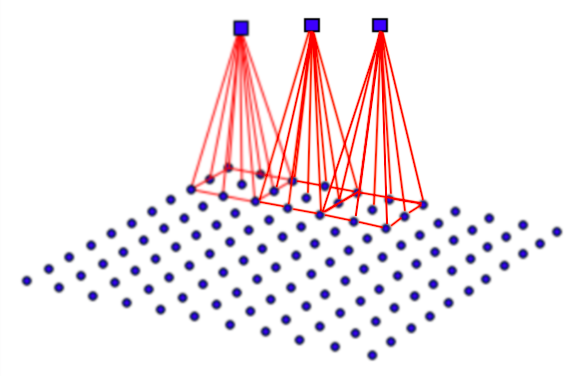
\includegraphics[width = 0.8\linewidth, height=3.3cm]{aplicacaostride.png}
   \caption {Exemplo de aplicação de pooling a uma imagem representada por pixeis}
   \end{subfigure}

\end{figure}

Num exemplo mais concreto, em baixo, podemos ver uma imagem cujas dimensões são 30 x 30, essa imagem foi tratada com uma janela deslizante de 3 x 3 e um stride de 3 nos eixos x e y resultando em 100 imagens a serem processadas pelo filtro escolhido.\newline
Como já foi referido cada filtro recebe uma sub-imagem correspondente aos pixeis abrangidos pela janela deslizante e devolve um valor, cada valor devolvido será posteriormente recolhido pela ordem em que cada sub-imagem foi filtrada de forma a refazer a figura com as caracteristicas obtidas através dos filtros. Em baixo podemos observar um esquema resumido de todo o processo de pooling.  

\begin{figure}[H]

  \centering
  \captionsetup{justification=centering}

  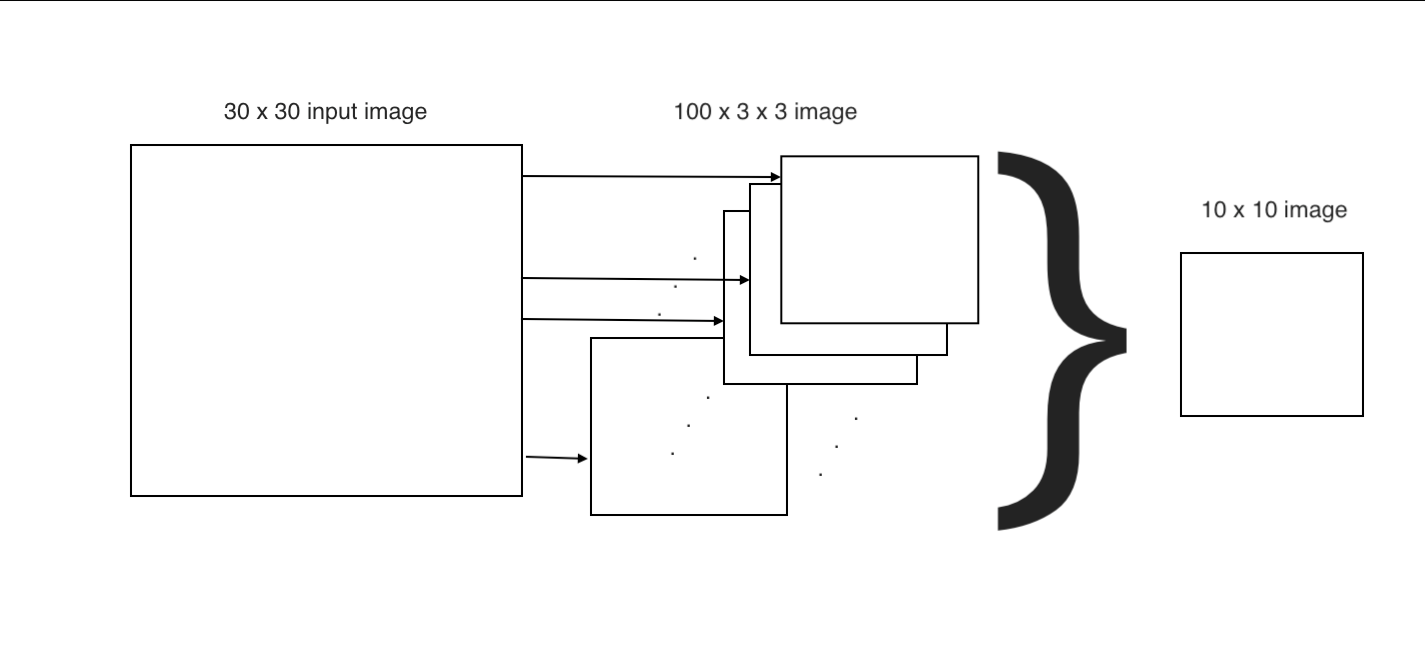
\includegraphics[width = 0.8\textwidth]{pooling.png}
  
  \caption {Esquema básico de pooling}

\end{figure}

\subsection{Poolings Clássicos}\hfill\newline
\hfill\newline
\label{subsec:poolingClassico}

Existem alguns pooling classicos que são comummente usados como o "max-pooling", "min-pooling", "average-pooling" e "maximum centered pooling", todos eles serão em seguida explicados.

\subsubsection{Max-Pooling}\hfill\newline
  \hfill\newline
  O max pooling trata-se de um filtro aplicado a uma imagem que devolve o valor máximo dessa imagem, isto é, como cada imagem consiste num conjunto de pixeis cujos valores variam dentro do intervalo de números inteiros [0,255] o max-pooling vai devolver o valor mais alto contido na imagem\cite{ref8}. Seja $A$ uma janela de pixeis que representa uma parte de uma imagem, a formula deste filtro aplicado a $A$ é a seguinte:\hfill\newline
  \hfill\newline
  $max\_pooling(A) = max(A)$
  \hfill\newline
  \hfill\newline
  Um exemplo deste tipo de filtro pode ser visualizado em baixo.

  \begin{figure}[H]

    \centering
    \captionsetup{justification=centering}

    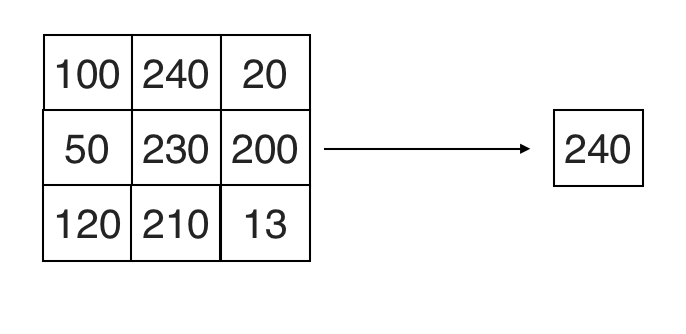
\includegraphics[width = 0.8\textwidth]{maxpooling.png}
    
    \caption {Exemplo de Max-Pooling}

  \end{figure}


\subsubsection{Min-Pooling}\hfill\newline
  \hfill\newline
  O min-pooling trata-se de um filtro aplicado a uma imagem que devolve o valor minimo contido nessa mesma imagem, isto é, dos valores dos pixeis da imagem é devolvido o menor. Seja $A$ uma janela de pixeis  que representa uma parte de uma imagem, a formula deste filtro aplicado a $A$ é a seguinte:\hfill\newline
  \hfill\newline
  $min\_pooling(L) = min(A)$
  \hfill\newline
  \hfill\newline
  Em baixo pode-se observar um exemplo deste filtro.

  \begin{figure}[H]

    \centering
    \captionsetup{justification=centering}

    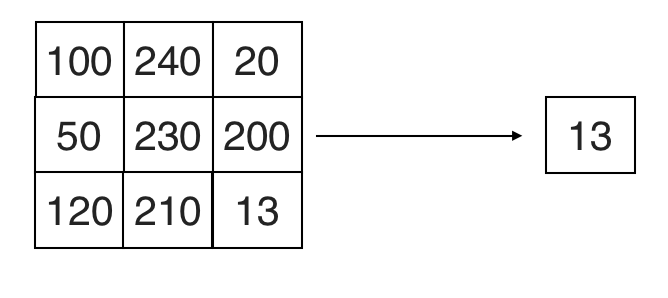
\includegraphics[width = 0.8\textwidth]{minpooling.png}
    
    \caption {Exemplo de Min-Pooling}

  \end{figure}


\subsubsection{Average Pooling}\hfill\newline
  \hfill\newline
  O average pooling trata-se de um filtro aplicado a uma imagem que devolve o valor médio dos pixeis dessa imagem, isto é, os valores de todos os pixeis são somados e posteriormente são divididos pelo número de pixeis existentes na imagem para obter uma média por pixel\cite{ref8}. Seja $A$ uma janela de pixeis de uma parte de uma imagem com dimensões $L1$ e $L2$, a formula deste filtro aplicado a $A$ é a seguinte:\hfill\newline
  \hfill\newline
  $average\_pooling(A) = \frac{\sum_{i=0}^{L1}\sum_{j=0}^{L2} A_{ij}}{L1*L2}$
  \hfill\newline
  \hfill\newline
  Um exemplo deste filtro pode ser visualizado em baixo.

  \begin{figure}[H]

    \centering
    \captionsetup{justification=centering}

    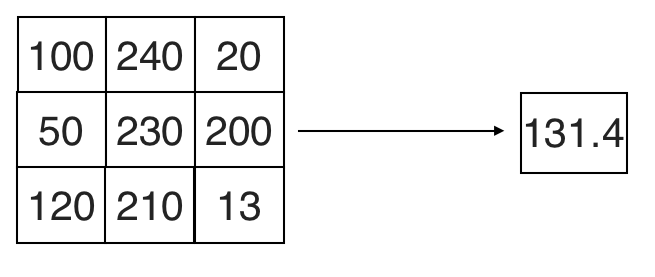
\includegraphics[width = 0.8\textwidth]{avgpooling.png}
    
    \caption {Exemplo de Average Pooling}

  \end{figure}


\subsubsection{Maximum Centered Pooling}\hfill\newline
  \hfill\newline
  O maximum minus average pooling trata-se de um filtro aplicado a uma imagem que devolve o valor médio dessa imagem subtraido ao valor máximo da mesma, isto é, primeiro acha-se a média dos pixeis da imagem e o valor máximo de todos esses pixeis e devolve-se a diferença entre o valor máximo encontrado e a média dos valores de todos os pixeis da imagem.Seja $A$ uma janela de pixeis de uma parte de uma imagem com dimensões $L1$ e $L2$, a formula deste filtro aplicado a $A$ é a seguinte:\hfill\newline
  \hfill\newline
  $max\_centered\_pooling(A) = max(A) - \frac{\sum_{i=0}^{L1}\sum_{j=0}^{L2} A_{ij}}{L1*L2}$
  \hfill\newline
  \hfill\newline
  Em baixo é apresentado um exemplo simples da aplicação deste filtro.

  \begin{figure}[H]

    \centering
    \captionsetup{justification=centering}

    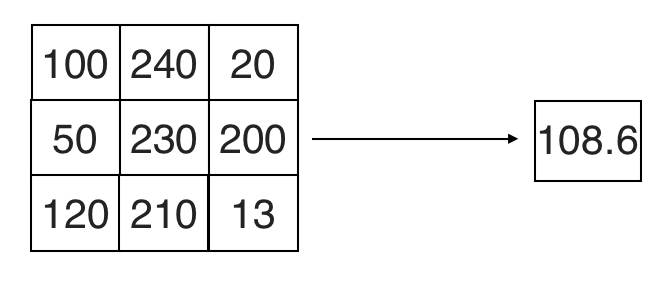
\includegraphics[width = 0.8\textwidth]{maxavgpooling.png}
    
    \caption {Exemplo de Maximum Centered Pooling}
  \end{figure}


\subsection{Poolings Exóticos}
\label{subsec:poolingExotico}

Existem também alguns poolings exóticos definidos especificamente para a base de dados que possuimos. Estes não funcionam da mesma maneira que os classicos uma vez que se baseiam em caracteristicas das imagens do dataset. \newline
Como o dataset é constituido de imagens do número 3 e do número 8 e a diferença na representação dos mesmos, de forma simplista, pode ser entendida com se tratando de que no oito temos dois circulos fechados e no três temos dois circulos com cerca de um quarto dos mesmos por concluir, sendo a junção dos circulos sobreposta de igual forma com se pode ver nas figuras abaixo.

\begin{figure}[H]

  %\centering
  \captionsetup{justification=centering}
  \begin{subfigure}{.5\textwidth}
  \centering
  
\includegraphics[width = 0.4\linewidth, height=3cm]{3.png}
  \end{subfigure}
  \begin{subfigure}{.5\textwidth}
  \centering
   
\includegraphics[width = 0.4\linewidth, height=3.3cm]{8.png}
   \end{subfigure}
  \caption {Representação dos números 3 e 8}
\end{figure}

Isto fornece-nos algumas ideias sobre os tipos de filtros que se podem criar tendo em conta esta simplificação das diferenças dos mesmos.


\subsubsection{ Diagonal and Vertical Average Pooling}\hfill\newline
  \hfill\newline
  Neste primeiro filtro a ideia subjacente passa por, tentar utilizar a diferença dos valores dos pixeis do oito e do 3 verticalmente e diagonalmente tal como se pode ver nas figuras abaixo que identificam o que esperamos encontrar. \hfill\newline

  \begin{figure}[H]

      %\centering
      \captionsetup{justification=centering}
      \begin{subfigure}{.5\textwidth}
        \centering
        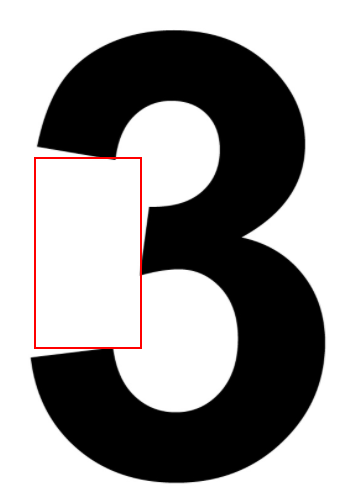
\includegraphics[width = 0.4\linewidth, height=3cm]{3_1.png}
        \end{subfigure}
        \begin{subfigure}{.5\textwidth}
        \centering
         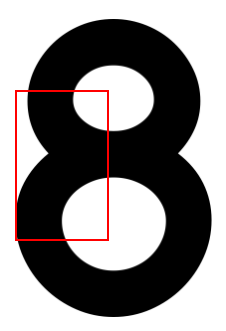
\includegraphics[width = 0.4\linewidth, height=3.3cm]{8_1.png}
      \end{subfigure}
      \begin{subfigure}{.5\textwidth}
        \centering
        
\includegraphics[width = 0.5\linewidth, height=3.5cm]{3_2.png}
        \end{subfigure}
        \begin{subfigure}{.5\textwidth}
        \centering
         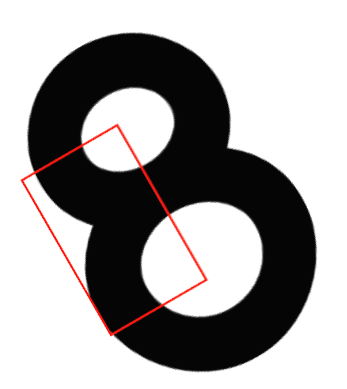
\includegraphics[width = 0.5\linewidth, height=3.8cm]{8_2.png}
      \end{subfigure}
      \caption {Representação do objetivo a identificar como o filtro sobre os números 3 e 8}
  \end{figure}

  A pensar neste tipo de abordagem este filtro soma os eixos diagonal (sentido descendente da esquerda para a direita) e vertical da janela recebida e divide os mesmos pelo número de elementos somados. Seja $A$ a janela de dimensões $size\_x$ e $size\_y$. As seguintes formulas mostram os passos para a realização do processo.\newline
  Posição inicial da lista vertical:\hfill\newline
  \hfill\newline
  $p\_vertical = size\_x : 2$, em que o valor p\_vertical é arredondado ás unidades.\hfill\newline
  \hfill\newline
  Posição inicial da lista diagonal:\hfill\newline
  \hfill\newline
  $p\_diagonal = 0$\hfill\newline
  \hfill\newline
  Deve existir um elemento que dite a linha da matriz a consultar começando inicializado a 0:\hfill\newline
  \hfill\newline
  $linha = 0$\hfill\newline
  \hfill\newline
  Deve ainda existir 1 lista para armazenar os pixeis verticais e diagonais, cujo comprimento é $L = 0$.\hfill\newline
  \hfill\newline
  $lista = []$\hfill\newline
  \hfill\newline
  A cada iteração a lista com os pixeis diagonais e verticais, que no inicio do processo se encontra vazia é atualizada acrescentando dois elementos da matriz $A$, fazendo com que o seu comprimento $L$ aumente também em 2 unidades.Adicionalmente a variável linha também aumenta em 1 unidade.\hfill\newline
  \hfill\newline
  $lista(k+1) = lista(k) + [ A_{p\_diagonal,linha}] + [ A_{p\_vertical,linha}]$\hfill\newline
  $L(k+1) = L(k) + 2$\hfill\newline
  $linha(k+1) = linha(k) + 1$\hfill\newline
  \hfill\newline
  No final é realizada a soma dos elementos da lista e a divisão  desta soma pelo número de elementos da mesma.\hfill\newline
  \hfill\newline
  $media = \frac{\sum_{i=0}^{L} lista_i}{L}$\hfill\newline
  \hfill\newline

  A variável media é devolvido pelo filtro como o resultado do processamento da janela.


\subsubsection{Diagonal and Vertical Max Centered Pooling}\hfill\newline
  \hfill\newline
  Á semelhança do filtro anterior este filtro também pretende usar a diagonal e a vertical do vetor representativo da janela deslizante, a diferença é que este subtrai a média, que é calculada da mesma forma que na função anterior, ao valor máximo encontrado na diagonal e vertical da janela representada pelo vetor. Assim, reaproveitando todas as definições anteriormente apresentadas o resultado devolvido por este filtro é:\hfill\newline
  \hfill\newline
  $max\_centered = max(lista) - media$



\subsubsection{Diagonal and Vertical Max Pooling}\hfill\newline
  \hfill\newline
  Este filtro parte do principio que as imagens representativas dos números 3 e 8 podem ser dadas rotacionadas em qualquer direção e para tentar mitigar esse problema são calculas ambas as diagonais e a vertical colecionando-as em arrays distintos, verifica qual o valor mínimo de cada um dos arrays colecionados e posteriormente devolve o maximo valor dos 3 anteriormente obtidos. As definições das seguintes formulas são dadas pela ordem de implementação:\hfill\newline 
  \hfill\newline
  Posição inicial da lista vertical $V1 $:\hfill\newline
  \hfill\newline
  $p\_vertical = size\_x : 2$, em que o valor p\_vertical é arredondado ás unidades.\hfill\newline
  \hfill\newline
  Valor a ser usado para calcular as posições dos pixeis de ambas as listas diagonais $D1$ e $D2$:\hfill\newline
  \hfill\newline
  $p\_diagonal = 0$\hfill\newline
  \hfill\newline
  Deve existir um elemento que dite a linha da matriz a consultar começando inicializado a 0:\hfill\newline
  \hfill\newline
  $linha = 0$\hfill\newline
  \hfill\newline
  Devem ainda existir 3 listas para armazenar os pixeis verticais e diagonais, cujos comprimentos são 0 aquando da sua criação.\hfill\newline
  \hfill\newline
  $V1 = []$\hfill\newline
  $D1 = []$\hfill\newline
  $D2 = []$\hfill\newline
  \hfill\newline
  A cada iteração as listas são incrementadas em 1 elemento. Adicionalmente a variável linha também aumenta em 1 unidade.\hfill\newline
  \hfill\newline
  $V1(k+1) = V1(k) + [ A_{p\_vertical,linha}]$\hfill\newline
  $D1(k+1) = D1(k) + [ A_{p\_diagonal,linha}]$\hfill\newline
  $D2(k+1) = D2(k) + [ A_{size\_x-(p\_diagonal+1),linha}]$\footnote{Note-se que é necessário somar uma unidade a $p\_diagonal$ uma vez que o primeiro elemento de A se encontra na posição 0 fazendo com que o último elemento de uma linha da matriz se encontre numa posição múltipla de $size\_x-1$ e não de $size\_x$}\hfill\newline
  $linha(k+1) = linha(k) + 1$\hfill\newline
  \hfill\newline
  No final é devolvido o pixel com valor máximo das 3 listas criadas.\hfill\newline
  \hfill\newline
  $maximum = max(max(max(V1),max(D1)),max(D2))$\hfill\newline
  \hfill\newline
\newpage

\subsubsection{Diagonal and Vertical Min Average Pooling}\hfill\newline
  \hfill\newline
  Á semelhança do filtro anterior, este filtro calcula 3 arrays correspondentes ás diagonais e á vertical. Em seguida realiza a média de cada um dos arrays e devolve a menor média. Assim, reaproveitando as definições anteriormente feitas sobre os arrays $V1$, $D1$ e $D2$ e sobre as respetivas atualizações a cada iteração temos as seguintes definições:\hfill\newline
  Para cada lista é necessário calcular a média. Note-se que cada lista possui o mesmo comprimento pois foi recolhido 1 pixel por linha para cada uma. Seja $Dim1$ a dimensão da lista $V1$ assim:\hfill\newline
  \hfill\newline
  $M1 = \frac{\sum_{i=0}^{Dim1} V1_i}{Dim1}$ \hfill\newline
  $M2 = \frac{\sum_{i=0}^{Dim1} D1_i}{Dim1}$ \hfill\newline
  $M3 = \frac{\sum_{i=0}^{Dim1} D2_i}{Dim1}$ \hfill\newline
  \hfill\newline
  Por fim é realizada a escolha da menor média obtida. \hfill\newline
  \hfill\newline
  $menor\_media = min(min(M1,M2),M3)$ \hfill\newline
  \hfill\newline
